\chapter{Characterization: How we measured the actual grating performance, and accounted for differences}
In the previous chapter, we applied grating efficiency calculations to create and optimize the optical design of the REIXS emission spectrometer.  After having the design reviewed by an external consultant, who confirmed our resolution and efficiency predictions (TODO REF), we solicited bids from grating manufacturers and selected Bach Research to mechanically rule the six gratings.  Finally, we passed the optical requirements over to a consulting engineer to design the mechanics of the spectrometer, which would be responsible for positioning the entrance slit, gratings, and detector, as well as achieving and maintaining ultra-high vacuum conditions throughout the beam path.

We lamented back in Chapter 4 the lack of published experimental comparisons of grating efficiency -- particularly in the soft x-ray regime -- and hypothesized that this was because beamline scientists, on receiving new gratings, were often eager to put them into their beamline and start commissioning, rather than spend more time characterizing them.  Unfortunately\footnote{for us in our role as beamline staff}, the construction of the REIXS spectrometer was delayed by a series of serious mechanical design flaws and oversights.  Fortunately\footnote{for our interests in grating efficiency}, this setback provided us with lots of time to characterize the ruling quality and real-world diffraction efficiency of our gratings.  Even more fortunately, the characterization process alerted us to serious ruling errors with a few of the gratings, which would have dramatically affected the spectrometer's resolution and efficiency had they not been discovered.  In the end, our characterization of the gratings resulted in several beneficial outcomes:
\begin{itemize}
\item We were able to contribute another set of experimental comparisons to theoretical grating efficiency calculations.
\item We discovered a reason to be cautious when specifying nickel-coated gratings, despite nickel's apparently high reflectivity.
\item We discovered a serious ruling problem in the HEG grating, which nearly eliminated its ability to diffract in the useful orders, and sent it back to the manufacturer for re-coating and re-ruling.
\item We discovered substantial errors in the blaze angle (beyond the manufacturer's specified tolerance) for a few of the gratings; in the case of the HRHEG, the blaze angle was off by so much that we ended up using it as a temporary replacement for the HEG.
\end{itemize}

This chapter describes these results, based on atomic force microprobe (AFM) measurements of the groove profile and soft x-ray diffractometer measurements of the actual grating efficiency.  We also compare the calculated and measured grating efficiencies, and offer explanations for the differences.

\section{AFM measurements of the manufactured grating profile}
When we consider a grating like the HEG, with 2000 lines/mm and a blaze angle of 1.52$\deg$, it is clear that the physical size of the grooves is extremely small -- we're talking about little triangles 500nm wide and maybe 13nm tall.  Measuring the physical geometry is therefore actually impossible with visible light microscopes.

Atomic force microscopy (AFM) is an extremely high-resolution technique for measuring the topography of a surface.  It uses an extremely sharp-tipped mechanical probe mounted on a piezo-electrically-controlled cantilever to ``feel'' the surface (Figure \ref{afm}).  The tip can either be dragged across the surface (contact mode) or electronically oscillated near its resonance frequency (\emph{non-contact mode}) while measuring the change in amplitude, phase and frequency caused by the tip-sample atomic interaction forces.  In both cases, the accurate vertical position of the tip is measured with a laser beam reflected off the back of the cantilever -- using either an interferometer or a deflection meter -- and the horizontal position of the tip is scanned using piezo drivers.  The resolution of the best atomic force microscopes is sufficient to image individual atoms on a surface, although for measuring soft x-ray gratings we only need angstrom-level accuracy.

One limitation of AFM techniques is that it's easy to produce a two-dimensional map of the relative surface profile in arbitrary units, but difficult to accurately determine the absolute height.  In order to measure blaze angles of gratings, we need to measure the height difference from the bottom to the top of the grooves in absolute units, which requires calibration of the AFM using a height standard.  (Usually this is a gold mesh with an accurately-known wire size.)

After receiving the gratings from the manufacturer, we first imaged them using the AFM at the University of Saskatchewan Structural Sciences Centre (SSSC).  However, we weren't able to calibrate the $z$-axis for these measurements, so with the assistance of Dr. Eric Gullikson, we requested a complete set of measurements using the AFM at the Center for X-Ray Optics at the Lawrence Berkeley National Laboratory.

An example of an AFM scan is given in Figure \ref{5a}, where we show both the two-dimensional image (top) and a cross-section of heights perpendicular to the grooves (bottom), revealing the groove profile.  Although the grooves should be ideally uniform along their entire length, most of the AFM scans show profile variation across even one image (a distance of just a few micrometers).  To determine the average profile shape and average blaze angle, we integrated the two-dimensional image across the groove direction.  Since a single AFM scan only spans a few micrometers of the grating, we also need to be careful in extrapolating the results to the entire grating; therefore, we conducted multiple scans at the centre and the corners of the grating.

\begin{figure}[htbp] %  figure placement: here, top, bottom, or page
   \centering
   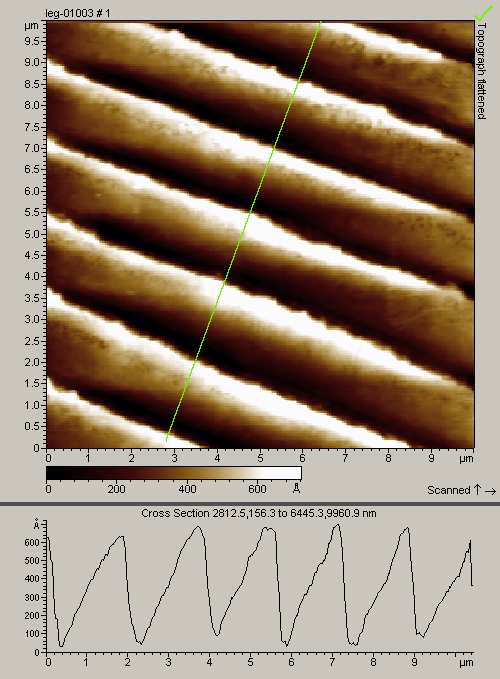
\includegraphics[width=6.5in]{Chapter5/5a_exampleAFM/afm_LEG_xsect1.png} 
   \caption{The Low Energy Grating has a smooth regular profile, shown in this example image measured using an Atomic Force Microprobe (AFM).}
   \label{5a}
\end{figure}

Figure \ref{5a} gives an example of the AFM output, for the LEG grating.  We present  groove profiles for all the gratings starting in Section \ref{gratingResults}, alongside a discussion of their effective diffraction performance.

\section{Diffractometer measurements of actual grating efficiency}

\subsection{Beamline 6.3.2 Diffractometer}
- describe machine

TODO: get paper and cite: http://ieeexplore.ieee.org/xpl/freeabs\_all.jsp?arnumber=4994440

\begin{figure}[htbp] %  figure placement: here, top, bottom, or page
   \centering
   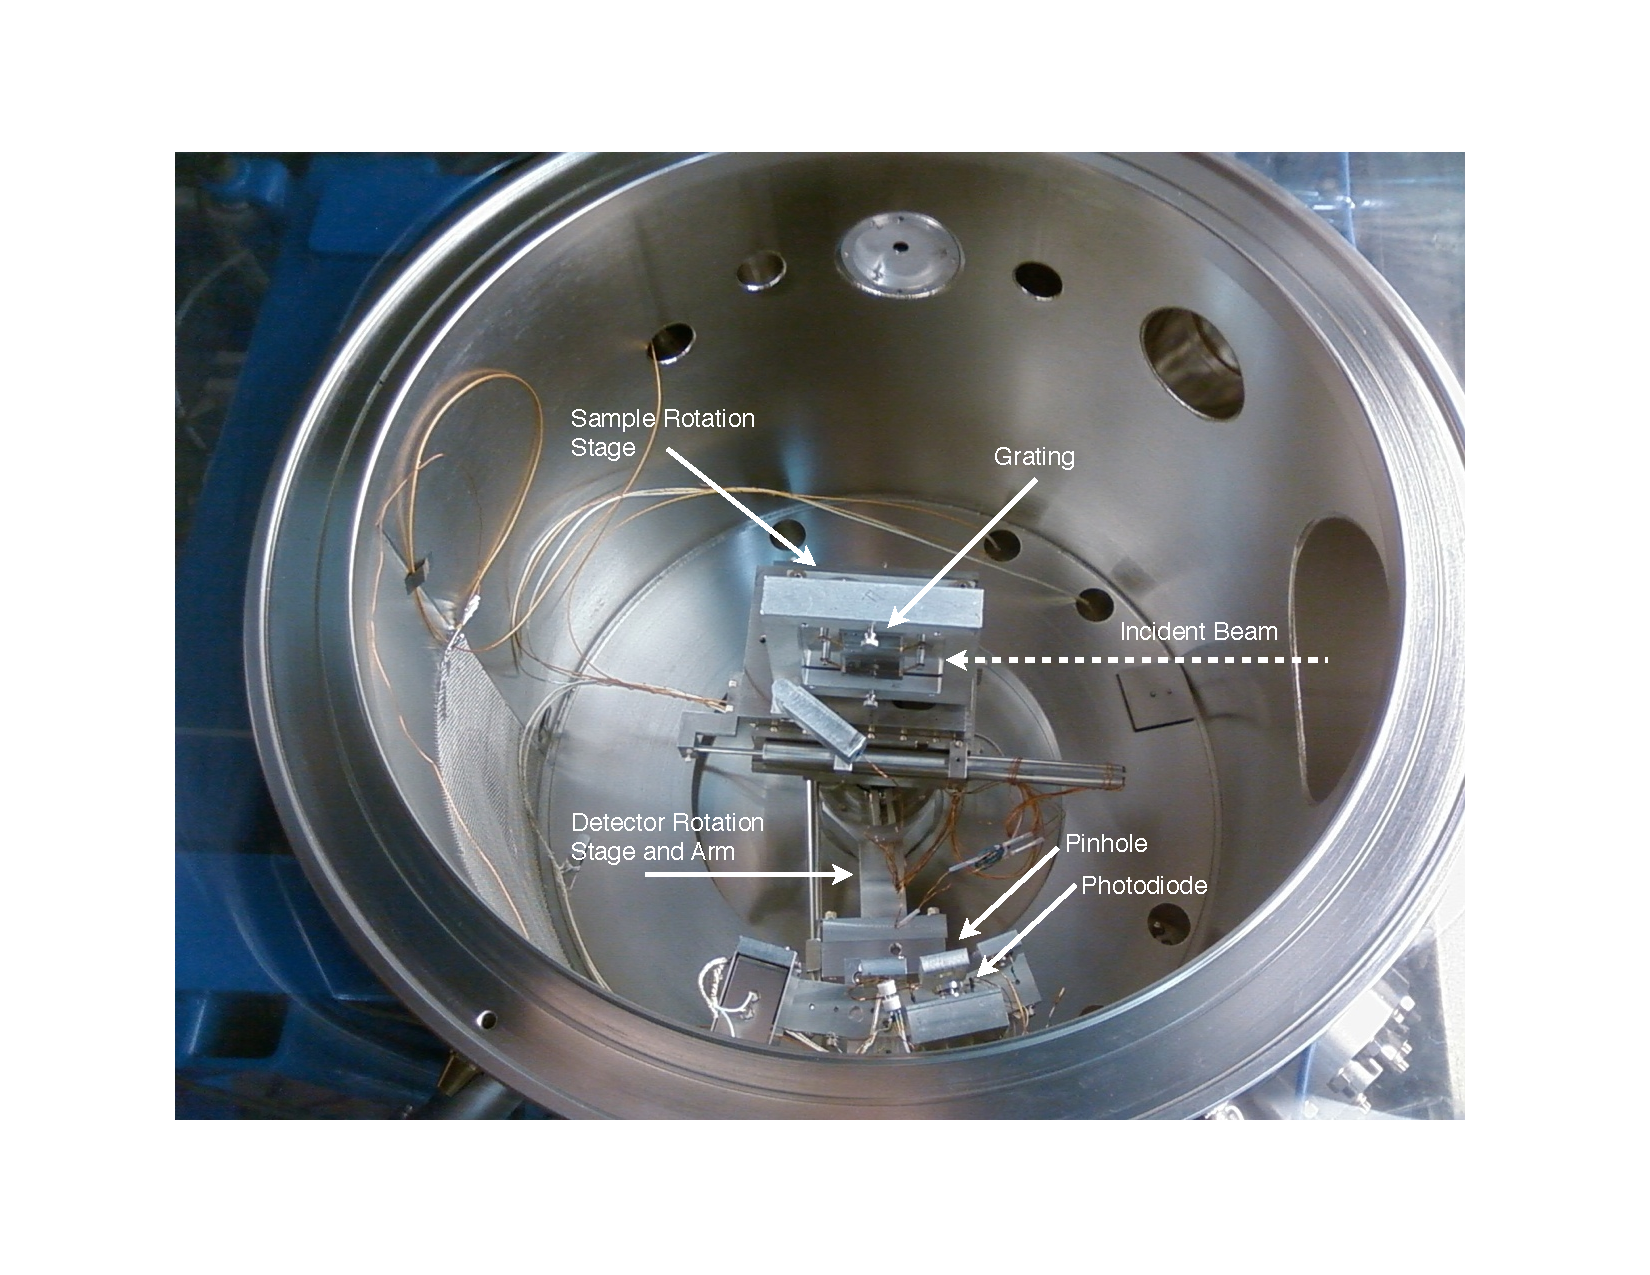
\includegraphics[width=7in]{Chapter5/5b_diffractometer/diffractometer_labelled.pdf} 
   \caption{The diffractometer on Beamline 6.3.2 at the Advanced Light Source allows for independently setting the angle of the gratings in the beam, and setting the angle of a pinhole photodiode detector.  Upstream, filters in the beamline are used to remove contamination from the higher-order light of the monochromator. }
   \label{5b}
\end{figure}

FIGURE 5b: picture of diffractometer tank with gratings positioned

- If you know groove density: can position to detector to correct angle as you scan energy. Otherwise, need to scan angle to find diffraction peak, and take eff. there.

DATA 5c: example angle scan at energies of interest

\begin{figure}[htbp] %  figure placement: here, top, bottom, or page
   \centering
   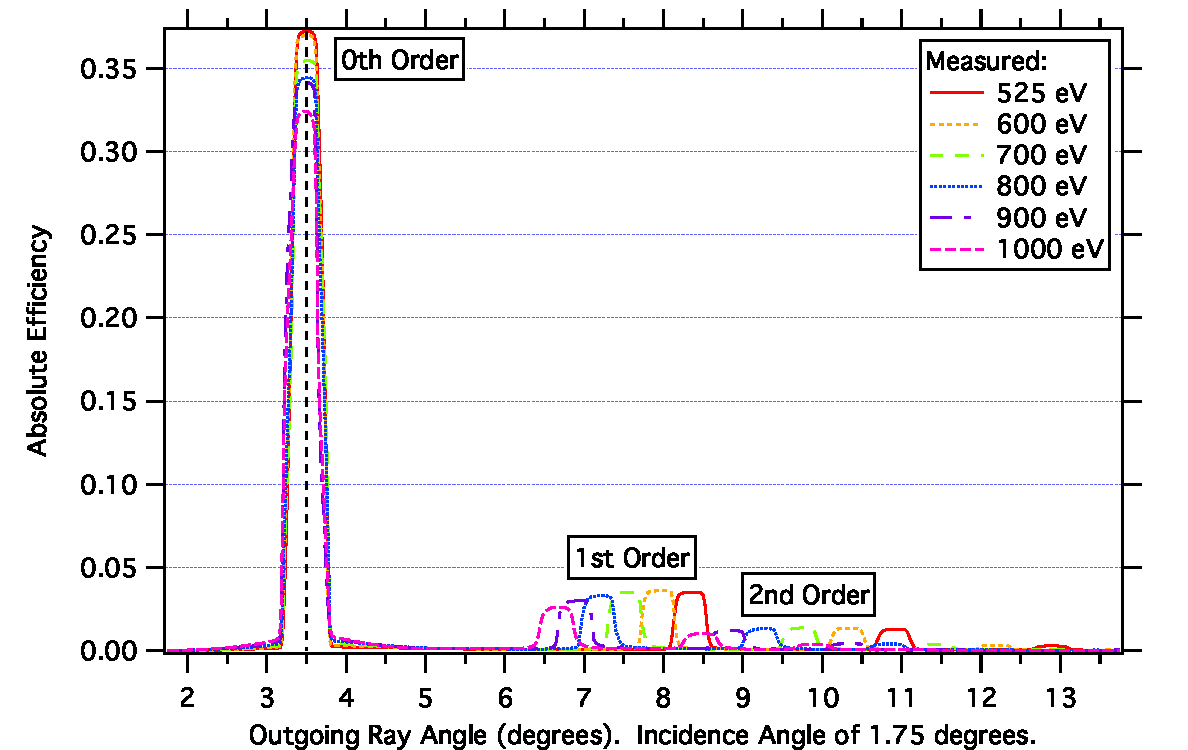
\includegraphics[scale=0.8]{Chapter5/5c_angleScan/5c.pdf} 
   \caption{The simplest diffractometer experiment scans the detector angle while illuminating the grating with a constant photon energy.  The diffraction orders are visible as peaks along the outgoing angle axis (here, measured up from the grating surface at 0 $\deg$).  The 0th order (reflection) peak is easily visible at twice the incident angle.  (Grating: HRHEG)}
   \label{5c}
\end{figure}

DATA: 5d example energy scan known groove density

\begin{figure}[htbp] %  figure placement: here, top, bottom, or page
   \centering
   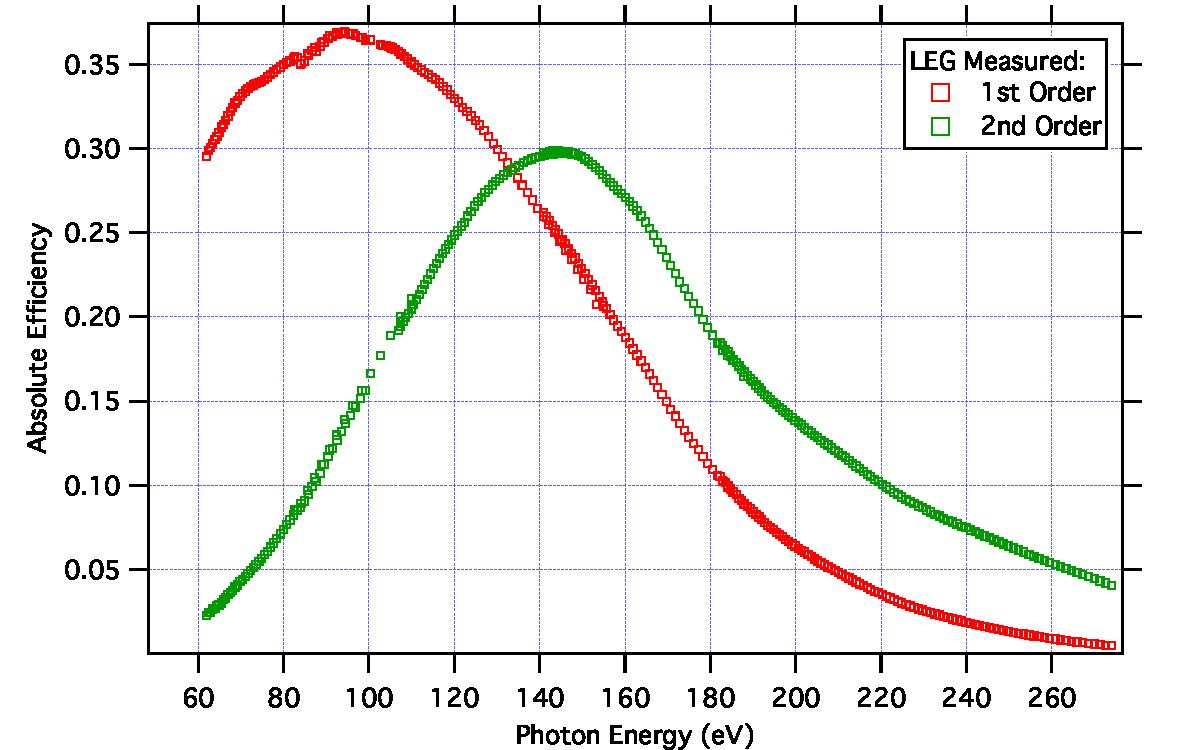
\includegraphics[scale=0.8]{Chapter5/5d_energyScan/5d_LEG.pdf} 
   \caption{When the groove density of a grating is accurately known, the detector angle can be scanned in synchronization to keep it on the diffraction peak as the incident photon energy is scanned.  This allows faster, continuous efficiency measurements as a function of  photon energy.  (Grating: LEG)}
   \label{5d}
\end{figure}

- mono: higher-order light contamination.  Uses filters in front of end station

\section{Real-world grating effects}
\label{realWorldEffects}
\subsection{Stray Radiant Energy}
http://gratings.newport.com/information/technotes/technote9.asp
\subsubsection{Surface roughness}
 (scattering: uniform decrease in efficiency)
  Other way to think about: periodic structures with \emph{many} frequency components. Diffract all over the place.
  
  TODO: Find reference and descriptive math...
  
          - Not modelled.  Accept a uniform constant reduction (usually about ~50\%) lower due to scattering.

\begin{figure}[htbp] %  figure placement: here, top, bottom, or page
   \centering
   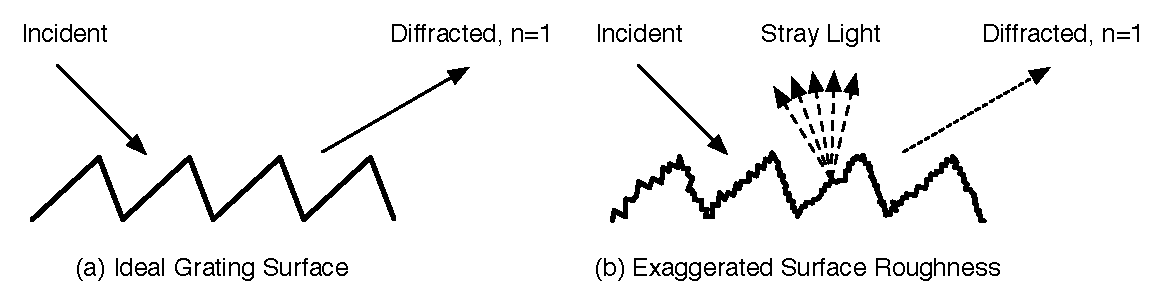
\includegraphics[scale=0.8]{Chapter5/5e_surfaceRoughness/5e.pdf} 
   \caption{Roughness of the grating surface scatters stray light outside the diffraction orders}
   \label{5e}
\end{figure}
       

\subsubsection{Dust, scratches, pinholes act as scattering centers}
\subsubsection{Irregularities in the groove position create ghost peaks}
\subsubsection{Irregularities along the groove direct light elsewhere}
reflect off axis... reduce periodicity... disrupt the perfect grating model. May be directed or diffuse.
\subsection{Blaze angle errors shift the efficiency peak}
\subsection{Coating oxidation changes the reflectivity spectrum}

\begin{figure}[htbp] %  figure placement: here, top, bottom, or page
   \centering
   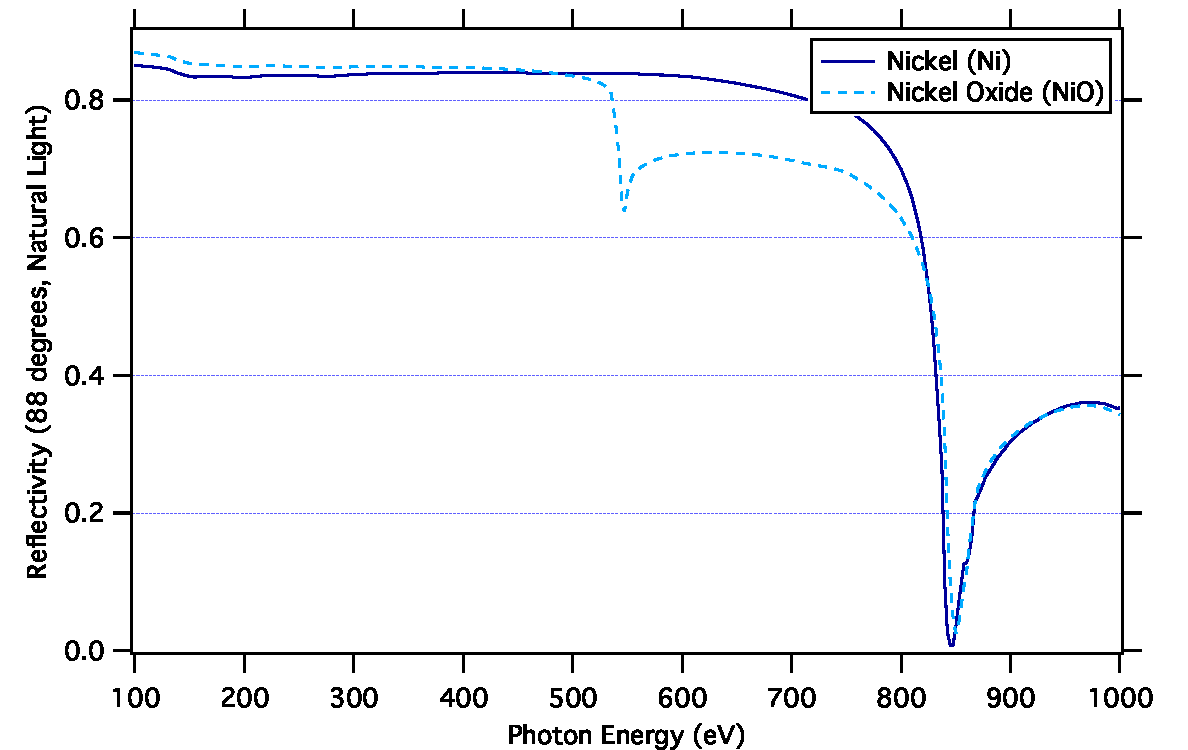
\includegraphics[scale=0.8]{Chapter5/5f_oxidized/Ni_NiO_reflec.pdf} 
   \caption{Unprotected Nickel quickly forms a surface oxide of NiO, which strongly reduces the reflectivity at the Oxygen edge (525eV) }
   \label{5f}
\end{figure}

\section{Grating results}
\label{gratingResults}
   : (and comparison to theoretical)
\subsection{LEG} (gold): profile clean; as expected; blaze angle off. [modelled]

\begin{figure}[htbp] %  figure placement: here, top, bottom, or page
   \centering
   \includegraphics[scale=0.8]{Chapter5/5y_afm/LEG.pdf} 
   \caption{AFM measurements of the Low Energy Grating (LEG) profile, averaged along the grooves (TODO um x TODO um).  The best-fit blaze angle is at the centre of the grating.}
   \label{5y-leg}
\end{figure}

\begin{figure}[htbp] %  figure placement: here, top, bottom, or page
   \centering
   \includegraphics[scale=0.8]{Chapter5/5x_comparison/LEG.pdf} 
   \caption{Theoretical and measured efficiency of the Low Energy Grating (LEG).}
   \label{5x-leg}
\end{figure}


\subsection{IMP} (nickel): Profile clean, blaze angle off [modelled].  Oxidized� Modelled as NI, layer of NiO.

TEST: NiO on top of Ni? layer thickness
Caveat: Henke data reflectivities are not correct at/near absorption edges... shouldn't totally match theoretical shape.

          - compare AFM and fitted
          
          scattering factor: http://www2.astro.psu.edu/~niel/astro485/xrayschool/schwartz-xray\_optics.pdf --> 1/sin(theta)

\begin{figure}[htbp] %  figure placement: here, top, bottom, or page
   \centering
   \includegraphics[scale=0.8]{Chapter5/5y_afm/IMP.pdf} 
   \caption{AFM measurements of the Impurity Grating (IMP) profile, averaged along the grooves (TODO um x TODO um).  The best-fit blaze angle is at the centre of the grating.}
   \label{5y-imp}
\end{figure}

\begin{figure}[htbp] %  figure placement: here, top, bottom, or page
   \centering
   \includegraphics[scale=0.8]{Chapter5/5x_comparison/IMP.pdf} 
   \caption{Theoretical and measured efficiency of the Impurity Grating (IMP).}
   \label{5x-imp}
\end{figure}


\subsection{MEG} (nickel): profile ok, blaze angle off [modelled].  Oxidized� Modelled as combination of NiO and NiO2.

\begin{figure}[htbp] %  figure placement: here, top, bottom, or page
   \centering
   \includegraphics[scale=0.8]{Chapter5/5y_afm/MEG.pdf} 
   \caption{AFM measurements of the Medium Energy Grating (MEG) profile, averaged along the grooves (TODO um x TODO um).  The best-fit blaze angle is at the centre of the grating.}
   \label{5y-meg}
\end{figure}

\begin{figure}[htbp] %  figure placement: here, top, bottom, or page
   \centering
   \includegraphics[scale=0.8]{Chapter5/5x_comparison/MEG.pdf} 
   \caption{Theoretical and measured efficiency of the Medium Energy Grating (LEG).}
   \label{5x-meg}
\end{figure}

\subsection{HEG} (Pt): almost no diffraction performance at all. AFM: revealed double-peak structure; not ruled correctly. Sent back to manuf.

\begin{figure}[htbp] %  figure placement: here, top, bottom, or page
   \centering
   \includegraphics[scale=0.8]{Chapter5/5y_afm/HEG.pdf} 
   \caption{AFM measurements of the High Energy Grating (HEG) profile, averaged along the grooves (TODO um x TODO um).  Severe ruling errors were apparent.  The profile wasn't sufficiently triangular to attempt to fit a blaze angle.}
   \label{5y-heg}
\end{figure}

\begin{figure}[htbp] %  figure placement: here, top, bottom, or page
   \centering
   \includegraphics[scale=0.8]{Chapter5/5x_comparison/HEG.pdf} 
   \caption{Theoretical and measured efficiency of the High Energy Grating (LEG).}
   \label{5x-heg}
\end{figure}

\subsection{HRMEG and HRHEG}

\begin{figure}[htbp] %  figure placement: here, top, bottom, or page
   \centering
   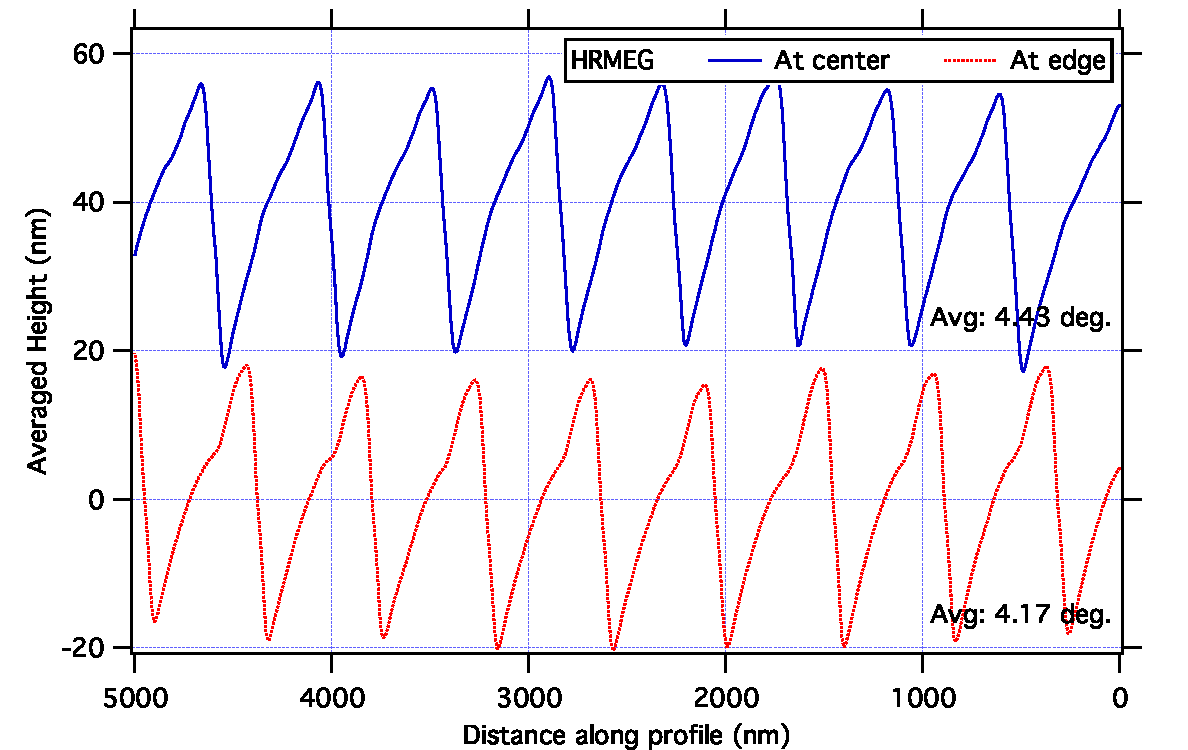
\includegraphics[scale=0.8]{Chapter5/5y_afm/HRMEG.pdf} 
   \caption{AFM measurements of the HighRes Medium Energy Grating (HRMEG) profile, averaged along the grooves (TODO um x TODO um).  The best-fit blaze angle is at the centre of the grating.}
   \label{5y-hrmeg}
\end{figure}

\begin{figure}[htbp] %  figure placement: here, top, bottom, or page
   \centering
   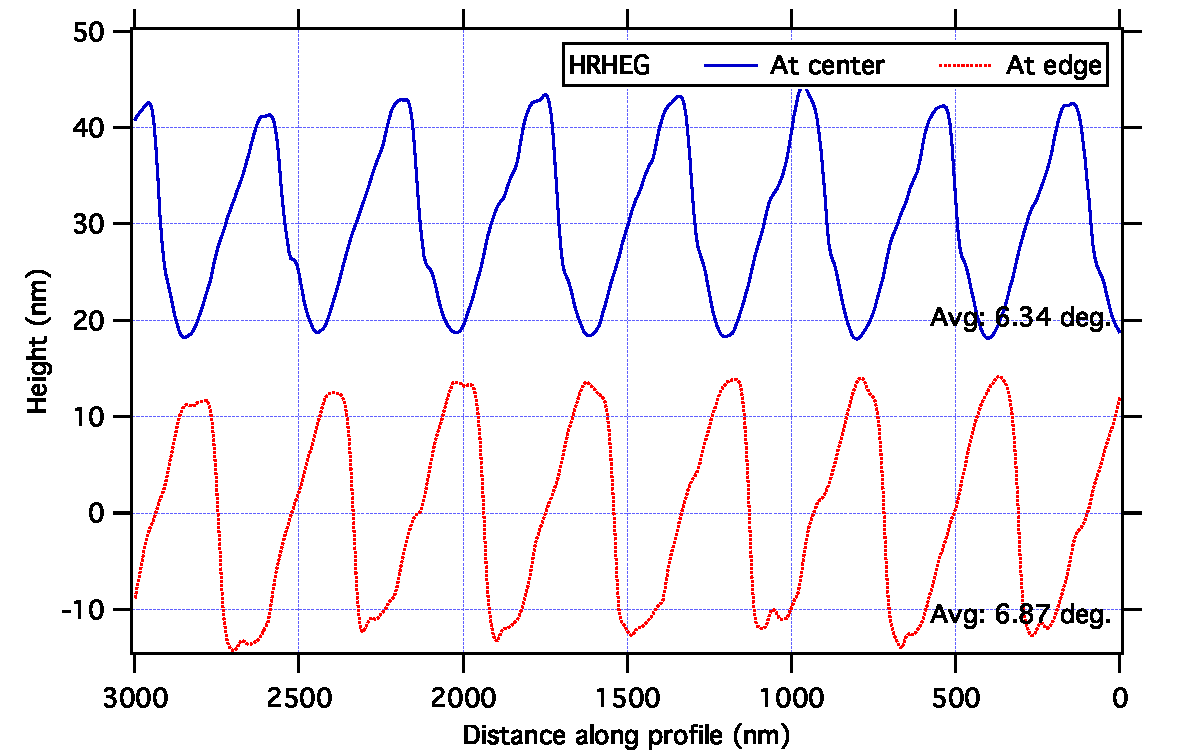
\includegraphics[scale=0.8]{Chapter5/5y_afm/HRHEG.pdf} 
   \caption{AFM measurements of the HighRes High Energy Grating (HRHEG) profile, averaged along the grooves (TODO um x TODO um).  The best-fit blaze angle is at the centre of the grating.}
   \label{5y-hrheg}
\end{figure}




 (Pt): blaze angles very off� Unsuitable for actual application in 3rd order.
          - Temporary plan: Using HRHEG (2600l/mm) in place of HEG (2000l/mm) since blaze angle error makes it suitable for use in 1st order.
               - DATA 5q: plot expected reduction in efficiency
               
